\documentclass[12pt]{article}
\usepackage{design_ASC}
\usepackage{amsmath}
\usepackage{mathtools}
\usepackage{listings}
\usepackage{graphicx}
\graphicspath{ {./} }

\newcommand\myeq{\stackrel{\mathclap{\normalfont\mbox{\;\;\;\;\small{$n\to\infty$}}}}{\;\;\;\;=\;\;}}

\setlength\parindent{0pt} %% Do not touch this

\title{Tema 2}

\author{Mihail Feraru\\
Grupa 142 - Structuri de Date\\
\textsc{Universiatea din Bucuresti}
}

\date{\today} %% Change "\today" by another date manually
%% -----------------------------
%% -----------------------------

%% %%%%%%%%%%%%%%%%%%%%%%%%%
\begin{document}
\setlength{\droptitle}{-5em}    
%% %%%%%%%%%%%%%%%%%%%%%%%%%
\maketitle

% --------------------------
% Start here
% --------------------------

% %%%%%%%%%%%%%%%%%%%
\section*{Problema 1}
% %%%%%%%%%%%%%%%%%%%

Fie $C$ un alfabet si $T$ arborele binar corespunzator codului sau optim pentru a coda un set de date oarecare. Pentru orice $c \in C$ consideram $c.freq$ numarul de aparitii al lui $c$ in setul de date ce trebuie codat, iar $d_T(c)$ lungimea codarii lui $c$. Prin cod optim ne referim la un cod cu urmatoarele doua proprietati:
\begin{itemize}
    \item[] \textbf{Proprietatea 1.} Oricum am alege doua reprezentari a doua elemente, niciuna din reprezentari nu este prefix pentru cealalta.
    \item[] \textbf{Proprietatea 2.} Costul codului definit astfel: $B(T) = \sum\limits_{c \in C} {c.freq \cdot d_T(c)}$ este minim.
\end{itemize}

Presupunem prin absurd ca exista un arbore binar $T'$ care nu este plin si corespunde unui cod optim pentru $C$. Cum $T'$ nu este plin, atunci exista un nod $x$ care are un singur fiu, $y$ care este asociat unui element din $C$. Fara a incalca \textbf{proprietatea 1}, putem interschimba $x$ si $y$, obtinem astfel un arbore notat $T''$. Cum $d_{T''}(y) < d_{T'}(y) \implies B(T'') < B(T')$, dar $T'$ corespunde unui cod optim, contradictie. \\

In concluzie, orice arbore arbore asociat unui cod optim trebuie sa fie plin. \qed

\section*{Problema 2}
Algoritmul de sortare quicksort ruleaza in cazul cel mai defavorabil in timp $O(n^2)$ din cauza alegerii nebalansate a pivotului. Recurenta generala este $T(n) = T(n - p - 1) + T(p - 1) + \Theta(n)$, unde $p$ reprezinta pozitia pivotului in sirul sortat, iar $\Theta(n)$ este timpul pentru efectuarea partitionarii. Observam ca daca pivotul ar coincide cu mediana sirului, recurenta se reduce la $T(n) = 2T([n/2]) + \Theta(n)$, care, aplicand teorema Master, ruleaza in timp $O(n \log{n})$ in cel mai nefavorabil caz. \\
Pentru a atinge complexitatea dorita este necesara determinarea medianei unui sir nesortat in $O(n)$. Acest lucru se poate realiza prin aplicarea algoritmului descris in \textit{Introduction to Algorithms, capitolul 9, sectiunea 2} implementat in metoda \textbf{RANDOMIZED-SELECT}. Pe scurt, este o adaptare a algoritmului quicksort care selecteaza a $n$-a valoare daca sirul s-ar sorta, fara ca acesta sa fie sortat.
In cele din urma, obtinem un quicksort care ruleaza in $O(n \log{n})$, insa selectarea pivotului in modul descris anterior aduce o constanta semnificativa in ecuatie, algoritmul devenind impractic intr-o gama larga de cazuri.

\section*{Problema 3}

Fie $x$ un nod dintr-un arbore binar de cautare. Definim $x.left$ si $x.right$ cei doi fii ai sai, $x.val$ valoarea sa, iar $NEXT(x)$ si $PREV(x)$ succesorul si predecesorul sau in parcurgerea in-order. \\

\textbf{Propozitia 3.} Predecesorul lui $x$ nu are fiu drept. \\
\textbf{Demonstratie.} Presupunem prin absurd ca exista un nod $y$ astfel incat $PREV(x).right = y$. Atunci, $y.val \geq PREV(x).val$ si $y.val \leq x.val$, deci $PREV(x) = y$, contradictie. \\

\textbf{Propozitia 4.} Succesorul lui $x$ nu are fiu stang. \\
\textbf{Demonstratie.} Presupunem prin absurd ca exista un nod $y$ astfel incat $NEXT(x).left = y$. Atunci, $y.val \leq NEXT(x).val$ si $y.val \geq x.val$, deci $NEXT(x) = y$, contradictie. \\

Consecinta directa a \textbf{propozitiilor 3 si 4} este ca predecesorul lui $x$ nu poate avea fiu drept, iar succesorul nu poate avea fiu stang. \qed
\\ \\ \\ \\ \\ \\ 
\begin{center}
    \textbf{Spatiu lasat gol in mod intentionat, problema 4 pe pagina urmatoare}
\end{center}

\newpage

\section*{Problema 4}
Vom folosi metoda Akra-Bazzi pentru rezolvarea recurentei. Forma generala este descrisa astfel:
\begin{equation*}
    T(x) = g(x) + \sum\limits_{i=1}^{k} {a_iT(b_ix+h_i(x))}
\end{equation*}
Pentru recurenta $T(n) = T(n / 2) + T(n / 3) + 1$ avem:
\begin{equation*}
    g(n) = 1 \in O(n^c), c \in \mathbb{R}, \;\; a_i = 1, \;\; h_i(n) = 0 \;\; \forall i \in \mathbb{N}, \;\;\; b_1 = \frac{1}{2}, \; b_2 = \frac{1}{3}, \;\; k = 2
\end{equation*}
Urmatorul pas al metodei este rezolvarea ecuatiei $\sum\limits_{i=1}^{k} {a_ib_i^p}=1 \Longleftrightarrow (\frac{1}{2})^p + (\frac{1}{3})^p = 1 \Longleftrightarrow 2^p + 3^p = 6^p$. Vom utiliza reprezentarea grafica pentu a obtine o aproximare cat mai buna a lui $p$. \\

\begin{center}
    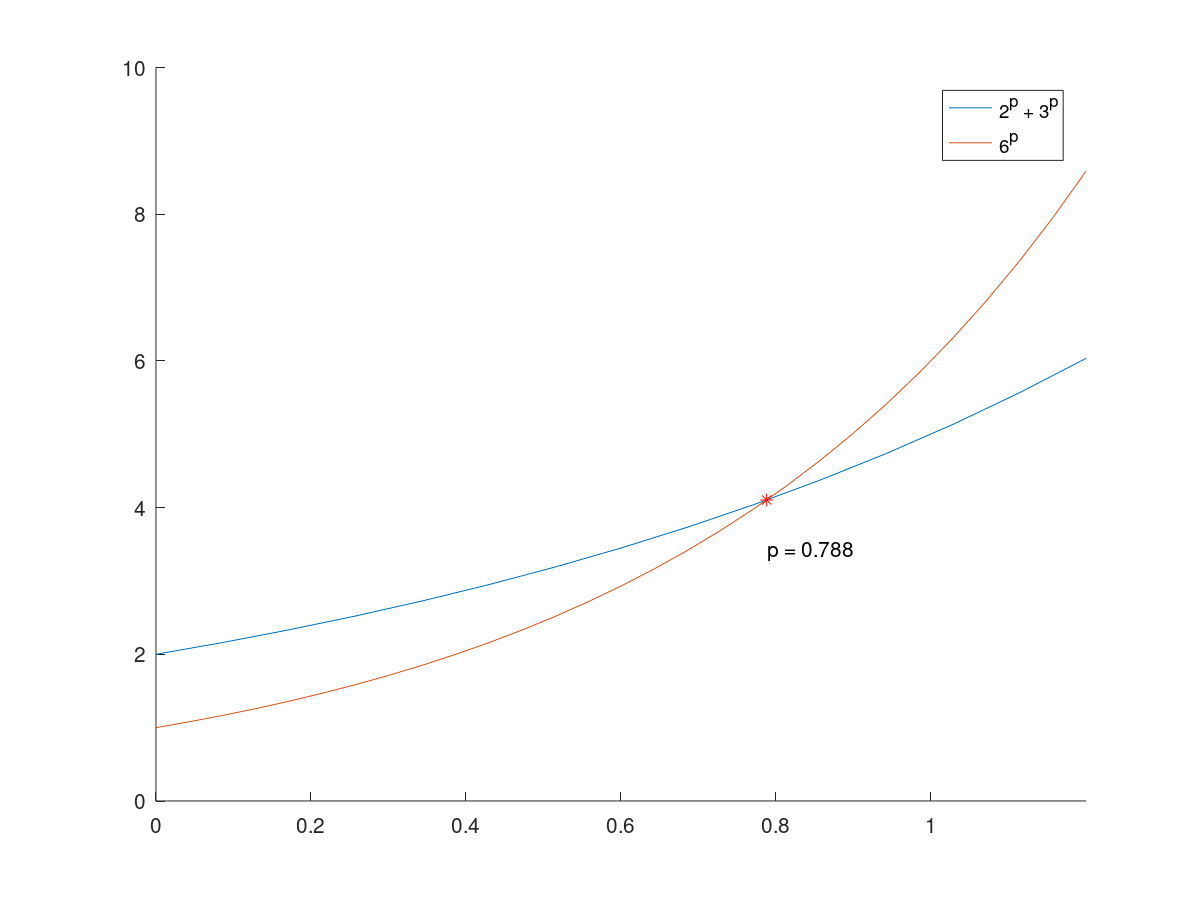
\includegraphics[scale=0.35]{ecuatie.png}
\end{center}

\begin{equation*}
    I = \int_{1}^{n} {\frac{g(n)}{u^{p+1}} du} = \int_{1}^{n} {\frac{1}{u^{p+1}} du} = \int_{1}^{n} {u^{-(p+1)} du} = \frac{u^{-p}}{-p}\Big|_1^n = \frac{1}{-pu^{p}}\Big|_1^n \myeq \;\;\; \frac{1}{p}
\end{equation*}
Conform metodei utilizate, $T(n)$ se incadreaza in clasa asimptotica:
\begin{equation*}
    T(n) \in \Theta(n^p (1 + I)) \Longleftrightarrow T(n) \in \Theta(n^p + \frac{n^p}{p}) \implies T(n) \in \Theta(n^p) = \Theta(n^{0.78})
\end{equation*}

\newpage
\subsection*{Compararea complexitatii lui T(n) cu diferite clase}
\begin{center}
    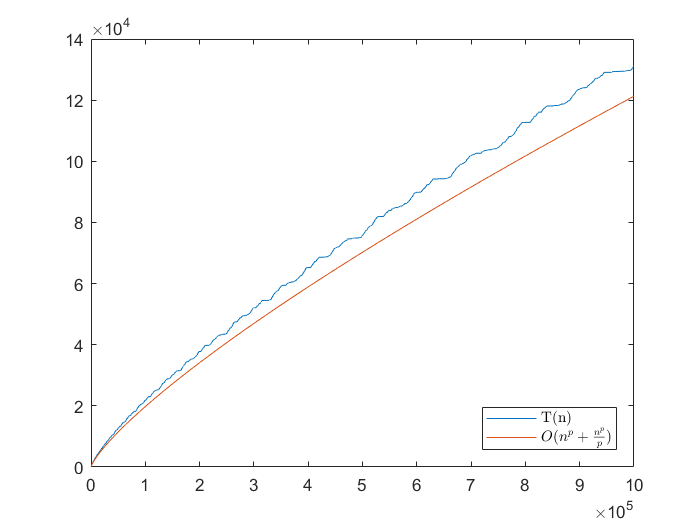
\includegraphics[scale=0.72]{compar1.png}
\end{center}
\begin{center}
    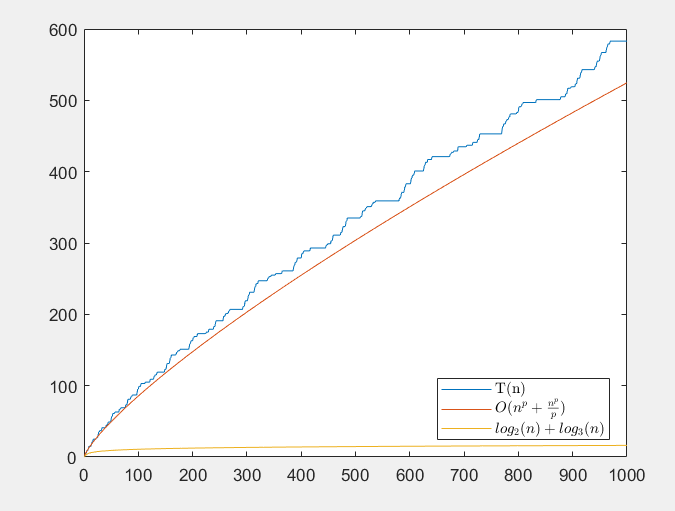
\includegraphics[scale=0.6]{compar2.png}
\end{center}
\begin{center}
    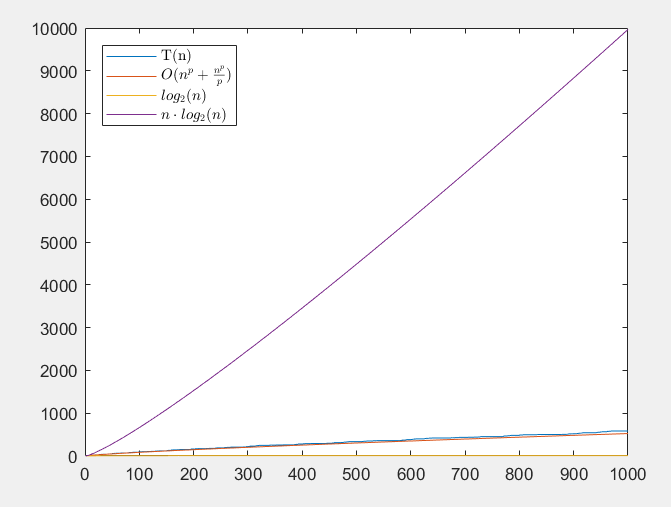
\includegraphics[scale=0.6]{compar3.png}
\end{center}

\end{document}
